\begin{frame}[fragile]{Exemplos de funções unimodais}

    \begin{figure}
        \centering

        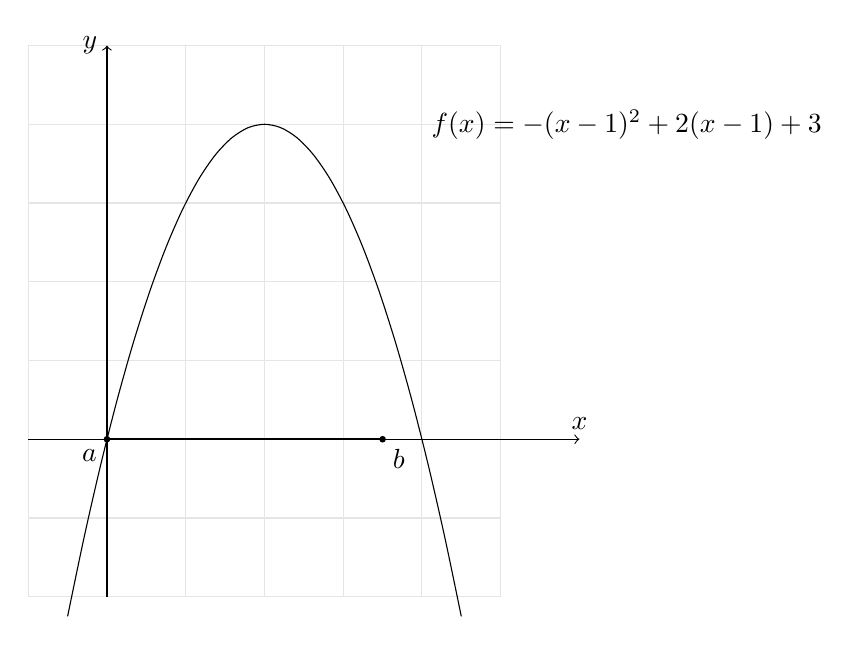
\begin{tikzpicture}
            \draw[gray!20] (-1, -2) grid (5, 5);

            \draw[smooth,domain=-0.5:4.5] plot (\x, {-(\x - 1)*(\x - 1) + 2*(\x - 1) + 3});
            \node[anchor=west] at (4, 4) { $f(x) = -(x - 1)^2 + 2(x - 1) + 3$ };

            \draw[->] (0,-2) -- (0, 5) node[anchor=east] { $y$ };
            \draw[->] (-1,0) -- (6, 0) node[anchor=south] { $x$ };

            \draw[thick] (0, 0) node[anchor=north east] { $a$ } -- (3.5, 0) node[anchor=north west] { $b$ };

            \fill (0,0) circle [radius=1.2pt];
            \fill (3.5,0) circle [radius=1.2pt];
        \end{tikzpicture}
    \end{figure}

\end{frame}

\begin{frame}[fragile]{Exemplos de funções unimodais}

    \begin{figure}
        \centering

        \begin{tikzpicture}
            \draw[gray!20] (-1, -2) grid (5, 5);

            \draw[smooth,domain=-0.5:4.5] plot (\x, {-(\x - 1)*(\x - 1) + 2*(\x - 1) + 3});
            \node[anchor=west] at (4, 4) { $f(x) = -(x - 1)^2 + 2(x - 1) + 3$ };
            \node[anchor=west] at (4, 3.25) { $m_1 = 1.16667, m_2 = 2.33333$ };
            \node[anchor=west] at (4, 2.5) { $f\left(m_1 + \left(\dfrac{m_2 - m_1}{2}\right)\right) = 3.88889$ };

            \draw[->] (0,-2) -- (0, 5) node[anchor=east] { $y$ };
            \draw[->] (-1,0) -- (6, 0) node[anchor=south] { $x$ };

            \draw[dashed] (1.16667, 0) node[anchor=north] { \scriptsize $m_1$ } -- (1.16667, 3.30556);
            \draw[dashed] (2.33333, 0) node[anchor=north] { \scriptsize $m_2$ } -- (2.33333, 3.88889);

\draw[thick] (0, 0) node[anchor=north east] { $a$ } -- (3.5, 0) node[anchor=north west] { $b$ };

            \fill (0,0) circle [radius=1.2pt];
            \fill (3.5,0) circle [radius=1.2pt];
        \end{tikzpicture}
    \end{figure}

\end{frame}

\begin{frame}[fragile]{Exemplos de funções unimodais}

    \begin{figure}
        \centering

        \begin{tikzpicture}
            \draw[gray!20] (-1, -2) grid (5, 5);

            \draw[smooth,domain=-0.5:4.5] plot (\x, {-(\x - 1)*(\x - 1) + 2*(\x - 1) + 3});
            \node[anchor=west] at (4, 4) { $f(x) = -(x - 1)^2 + 2(x - 1) + 3$ };
            \node[anchor=west] at (4, 3.25) { $m_1 = 1.94444, m_2 = 2.72222$ };
            \node[anchor=west] at (4, 2.5) { $f\left(m_1 + \left(\dfrac{m_2 - m_1}{2}\right)\right) = 3.99691$ };

            \draw[->] (0,-2) -- (0, 5) node[anchor=east] { $y$ };
            \draw[->] (-1,0) -- (6, 0) node[anchor=south] { $x$ };

            \draw[dashed] (1.94444, 0) node[anchor=north] { \scriptsize $m_1$ } -- (1.94444, 3.99691);
            \draw[dashed] (2.72222, 0) node[anchor=north] { \scriptsize $m_2$ } -- (2.72222, 3.4784);
            \draw[thick] (1.1667, 0) node[anchor=north east] { $a$ } -- (3.5, 0) node[anchor=north west] { $b$ };

            \fill (1.1667,0) circle [radius=1.2pt];
            \fill (3.5,0) circle [radius=1.2pt];
        \end{tikzpicture}
    \end{figure}

\end{frame}

\begin{frame}[fragile]{Exemplos de funções unimodais}

    \begin{figure}
        \centering

        \begin{tikzpicture}
            \draw[gray!20] (-1, -2) grid (5, 5);

            \draw[smooth,domain=-0.5:4.5] plot (\x, {-(\x - 1)*(\x - 1) + 2*(\x - 1) + 3});
            \node[anchor=west] at (4, 4) { $f(x) = -(x - 1)^2 + 2(x - 1) + 3$ };
            \node[anchor=west] at (4, 3.25) { $m_1 = 1.68519, m_2 = 2.20370$ };
            \node[anchor=west] at (4, 2.5) { $f\left(m_1 + \left(\dfrac{m_2 - m_1}{2}\right)\right) = 3.9585$ };
            \draw[->] (0,-2) -- (0, 5) node[anchor=east] { $y$ };
            \draw[->] (-1,0) -- (6, 0) node[anchor=south] { $x$ };

            \draw[dashed] (1.68519, 0) node[anchor=north] { \scriptsize $m_1$ } -- (1.68519, 3.90089);
            \draw[dashed] (2.20370, 0) node[anchor=north] { \scriptsize $m_2$ } -- (2.20370, 3.9585);
            \draw[thick] (1.1667, 0) node[anchor=north east] { $a$ } -- (2.72222, 0) node[anchor=north west] { $b$ };

            \fill (1.1667,0) circle [radius=1.2pt];
            \fill (2.72222,0) circle [radius=1.2pt];
        \end{tikzpicture}
    \end{figure}

\end{frame}
